\subsection{Színek}

%17
\begin{frame}
  Számtalan dolognak beállítható a színe CSS tulajdonságokkal, pl.:
  \begin{description}[m]
    \item[\texttt{color}] \hfill \\ Szöveg írásszíne
    \item[\texttt{background-color}] \hfill \\ Háttérszín
  \end{description}
  Szín, mint a tulajdonság értéke megadható:
  \begin{description}[m]
    \item[kulcsszavakkal] \hfill \\ Pl. \texttt{red} (vörös), 
    \texttt{green} (zöld), \texttt{blue} (kék), \texttt{white} (fehér), 
    \texttt{black} (fekete), \dots \\
    \hiv{\href{https://www.w3.org/TR/css-color-3/\#svg-color}%
    {140 szabványos színkód}}
    \item[Hexadecimálisan, RGB összetevőkkel] \hfill \\ Pl. 
    narancsszín: \texttt{\#ff7f00}, ahol \texttt{\#} jelzi a 16-os 
    számrendszerbeli alakot, \texttt{ff} a vörös (\kiemel{R}ed), 
    \texttt{7f} a zöld (\kiemel{G}reen) és \texttt{00} a kék 
    (\kiemel{B}lue) összetevő intenzitása 8 biten előjel nélkül, 
    fixpontosan. Additív színkeverés.
  \end{description}
\end{frame}

%18
\begin{frame}
  \begin{description}[m]
    \item[\texttt{rgb()} függvénnyel] \hfill \\ \texttt{rgb(red, 
    green, blue)}, ahol mindhárom összetevő lehet 0-255 közötti 
    decimális egész, vagy 0-100\%. Pl. \texttt{rgb(255,0,0)} vagy 
    \texttt{rgb(100\%, 0\%, 0\%)} vörös színt eredményez.
    \item[\texttt{rgba()} függvénnyel] \hfill \\ \texttt{rgb(red, 
    green, blue, alpha)}, ahol a színösszetevőket egy 
    átlátszóság érték követi ([0, 1]).
  \end{description}
  \vfill
  \begin{center}
    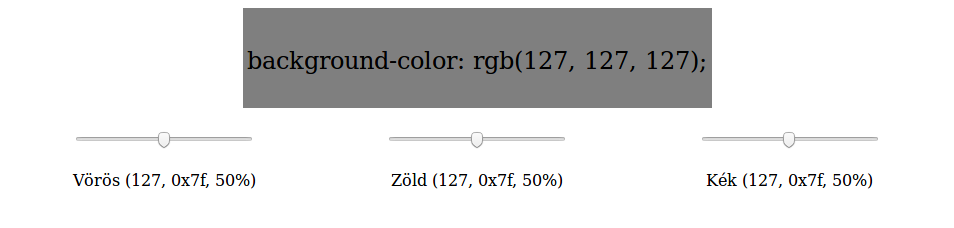
\includegraphics[scale=0.2]{szinek1.png}\\
    \textattachfile{szinek1.html}{szinek1.html}
  \end{center}
\end{frame}

%19
\begin{frame}
  \begin{description}[m]
    \item[\texttt{hsl()} függvénnyel] \hfill \\ \texttt{hsl(hue, 
    saturation, lightness)}, ahol \texttt{hue} az árnyalat, [0, 360] 
    fok közötti elfordulás a színkeréken. Pl. 0$^{\circ}$ a 
    vöröshöz, 120$^{\circ}$ a zöldhöz, 240$^{\circ}$ a kékhez 
    tartozik. \texttt{saturation} a telítettség, százalékban. A 0\% 
    a színinformáció hiányát (szürkeség) jelzi, 100\% a teljes 
    színezettséget. \texttt{lightness} a fényesség, szintén 
    százalékban. A 0\% mindig fekete, a 100\% mindig fehér színt ad.
    \item[\texttt{hsla()} függvénnyel] \hfill \\ A fentiek 
    kiegészülnek átlátszósággal.
  \end{description}
  \vfill
  \begin{center}
    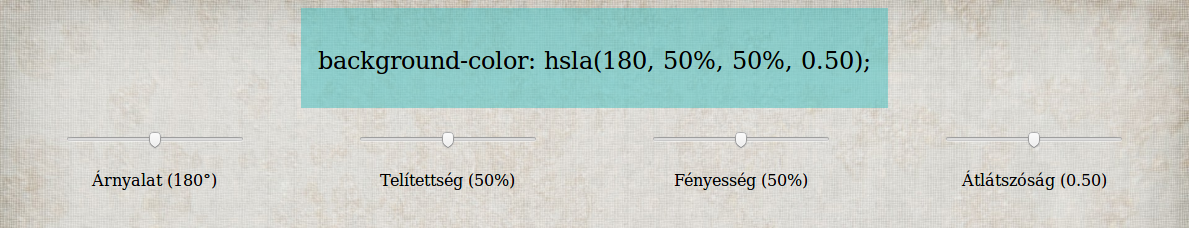
\includegraphics[scale=0.2]{szinek2.png}\\
    \textattachfile{szinek2.html}{szinek2.html}, \textattachfile{papir.jpg}{papir.jpg}
  \end{center}
\end{frame}

%_
\begin{frame}
  Az elemek átlátszósága az \texttt{opacity} tulajdonsággal is állítható [0, 1] intervallumban; a kisebb értékekhez nagyobb átlátszóság tartozik.
  \begin{exampleblock}{\textattachfile{atlatszosag1.html}{atlatszosag1.html} (\textattachfile{sze_logo.svg}{sze\_logo.svg}, \textattachfile{it_logo.svg}{it\_logo.svg})}
    \scriptsize
    \lstinputlisting[style=HTML,linerange={7-8},numbers=left,firstnumber=7]{atlatszosag1.html}
    \lstinputlisting[style=HTML,linerange={12-13},numbers=left,firstnumber=12]{atlatszosag1.html}
  \end{exampleblock}
  \begin{center}
    
\includegraphics[width=.5\textwidth]{atlatszosag1.png}
  \end{center}
\end{frame}

%20
\begin{frame}
  \begin{columns}[c]
    \column{0.5\textwidth}
      Induljon ki a \textattachfile{szinezes.html}{szinezes.html} 
      fájlból! Kapcsolja ezt össze egy külső stíluslappal, majd 
      érje el, hogy a jobb oldali ábrának megfelelő színekben 
      pompázzon! Próbáljon minél több féle szín megadási 
      módszert alkalmazni! Törekedjen a lehető legtömörebb CSS 
      szabályok megalkotására!
    \column{0.5\textwidth}
      \begin{exampleblock}{\textattachfile{szinezes-mo.html}{szinezes-mo.html}, 
        \textattachfile{szinezes-mo.css}{szinezes-mo.css}}
        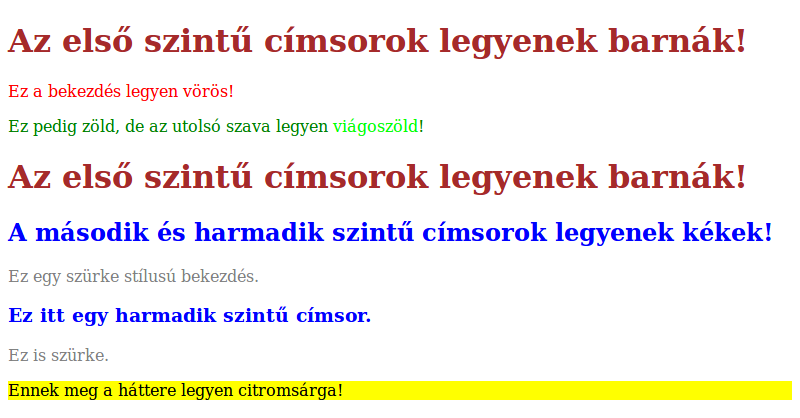
\includegraphics[width=\textwidth]{szinezes-mo.png}
      \end{exampleblock}
  \end{columns} 
\end{frame}
